\section{Standard di qualità}

	\subsection{ISO/IEC 9126}
	ISO/IEC 9126 è uno standard internazionale per valutare la qualità del software.\\%PLACEHOLDER mettere eventuale immagine dello standard
	Questo standard è diviso in quattro parti che vengono riportate di seguito.
		\subsubsection{Metriche per la qualità interna}
		Metriche che si applicano al software non eseguibile durante le fasi di progettazione e codifica. Permettono di individuare eventuali problemi che potrebbero influire sulla qualità finale del prodotto prima che venga realizzato un eseguibile. Grazie alle misure effettuate tramite le metriche interne è possibile prevedere il livello di qualità esterna e di qualità in uso del prodotto finale, poiché entrambe vengono influenzate dalla qualità interna.\\
		Viene rilevata tramite analisi statica. Idealmente la qualità interna determina la qualità esterna.
		\subsubsection{Metriche per la qualità esterna}
		Metriche applicabili al software in esecuzione che ne misurano il comportamento attraverso dei test, in funzione degli obiettivi stabiliti.\\
		Viene rilevata tramite analisi dinamica. Idealmente la qualità esterna determina la qualità in uso.
		\subsubsection{Metriche per la qualità in uso}
		Metriche applicabili solo al prodotto finito ed in uso in condizioni reali.\\
		La qualità in uso viene raggiunta solo se è stato raggiunto il livello di qualità interna e di qualità esterna.
		\subsubsection{Modello della qualità del software}
		Il modello di qualità del software suddivide la qualità in sei caratteristiche generali e varie sotto caratteristiche, misurabili attraverso delle metriche, utilizzate per fornire una scala ed un metodo per la misurazione. Di seguito sono riportate queste caratteristiche.
		\begin{figure}[H]
			\centering
			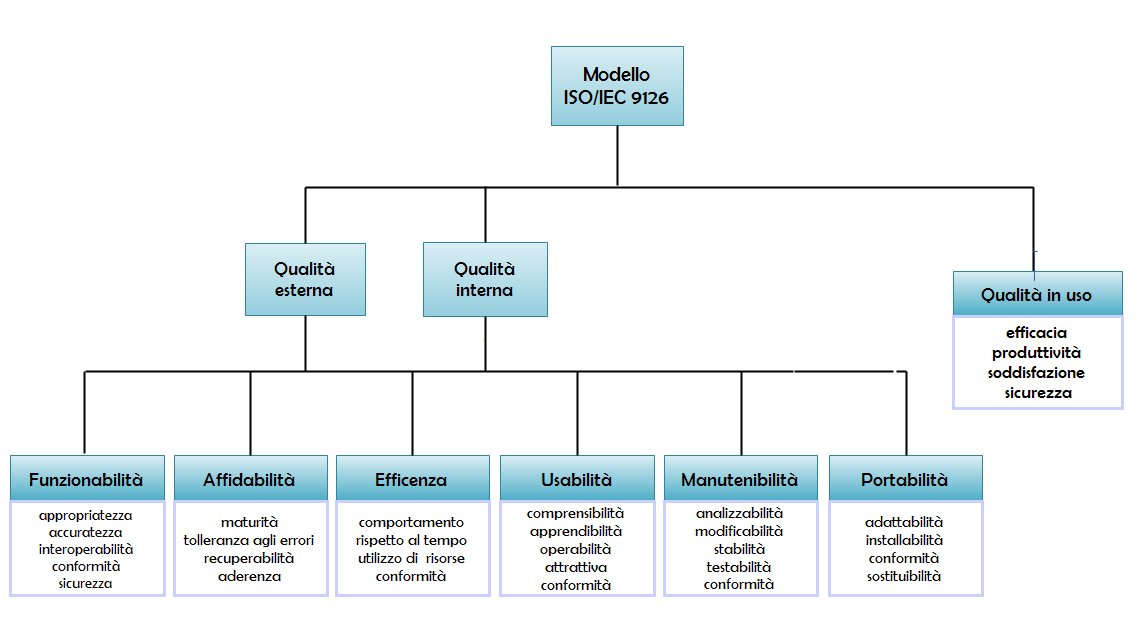
\includegraphics[scale=0.4]{res/images/iso9126.png}
			\caption{Qualità del software secondo ISO/IEC 9126}
		\end{figure}		
	
		\paragraph{Funzionalità}
		Capacità del software di soddisfare i requisiti, descritti nell'Analisi dei Requisiti, in un determinato contesto.\\
		Nello specifico il software deve soddisfare le seguenti caratteristiche:
		\begin{itemize}
			\item \textbf{Appropriatezza}: capacità di fornire funzioni appropriate per attività specifiche, che permettano di raggiungere gli obiettivi prefissati;
			\item \textbf{Accuratezza}: capacità di fornire i risultati concordati o la precisione richiesta;
			\item \textbf{Interoperabilità}: capacità di interagire ed operare con uno o più sistemi specificati;
			\item \textbf{Conformità}: capacità di aderire a standard;
			\item \textbf{Sicurezza}: capacità di proteggere informazioni e dati.
		\end{itemize}
		\paragraph{Affidabilità}
		Capacità del software di mantenere uno specifico livello di prestazioni quando usato in condizioni specificate.\\
		Nello specifico il software deve soddisfare le seguenti caratteristiche:
		\begin{itemize}
			\item \textbf{Maturità}: capacità di evitare il verificarsi di errori, malfunzionamenti o risultati non corretti;
			\item \textbf{Tolleranza agli errori}: capacità di mantenere livelli prefissati di prestazioni anche in presenza di malfunzionamenti o usi scorretti del prodotto finale;
			\item \textbf{Recuperabilità}: capacità di ripristinare un livello appropriato di prestazioni o di recupero di informazioni rilevanti a seguito di un malfunzionamento;
			\item \textbf{Aderenza}:  capacità di aderire a standard, regole e convenzioni che riguardano l'affidabilità.
		\end{itemize}
		\paragraph{Efficienza}
		Capacità del prodotto software di eseguire le proprie funzioni minimizzando il tempo necessario e sfruttando al meglio le risorse che necessita.\\
		Nello specifico il software deve soddisfare le seguenti caratteristiche:
		\begin{itemize}
			\item \textbf{Comportamento rispetto tempo}: capacità di fornire adeguati tempi di risposta, elaborazione e velocità di attraversamento in determinate condizioni;
			\item \textbf{Utilizzo di risorse}: capacità di utilizzo di quantità e tipo di risorse in maniera adeguata;
			\item \textbf{Conformità}: è la capacità di rispettare standard, regole e convenzioni riguardanti l'efficienza.
		\end{itemize}
		\paragraph{Usabilità}
		Capacità del prodotto software di essere compreso, appreso, usato e accettato dall'utente, quando usato sotto determinate condizioni.\newline
		Nello specifico il software deve soddisfare le seguenti caratteristiche:
		\begin{itemize}
			\item \textbf{Comprensibilità}: capacità di essere chiaro riguardo le proprie funzionalità e il proprio utilizzo;
			\item \textbf{Apprendibilità}: capacità di essere facilmente apprendibile dagli utenti;
			\item \textbf{Operabilità}: capacità di permettere all'utente di eseguire i suoi scopi e controllarne l'uso;
			\item \textbf{Attrattività}: capacità di essere piacevole all'utente che l'utilizza.
			\item \textbf{Conformità}: è la capacità di rispettare standard, regole e convenzioni riguardanti l'usabilità.
		\end{itemize}
		\paragraph{Manutenibilità}
		Capacità del software di essere modificato, al fine di aggiungere correzioni, miglioramenti o adattamenti.\\
		Nello specifico il software deve soddisfare le seguenti caratteristiche:
		\begin{itemize}
			\item \textbf{Analizzabilità}: capacità di essere facilmente analizzato al fine di localizzare un errore;
			\item \textbf{Modificabilità}: capacità di poter essere agevolmente modificato nel codice, nella progettazione o nella documentazione;
			\item \textbf{Stabilità}: capacità di evitare effetti indesiderati a seguito di una modifica;
			\item \textbf{Testabilità}: capacità di essere facilmente testato per validare le modifiche apportate.
			\item \textbf{Conformità}: è la capacità di rispettare standard, regole e convenzioni riguardanti la manutenibilità.
		\end{itemize}
		\paragraph{Portabilità}
		Capacità del software di essere trasportato da un ambiente di lavoro ad un altro, sia esso hardware che software.\\
		Nello specifico il software deve soddisfare le seguenti caratteristiche:
		\begin{itemize}
			\item \textbf{Adattabilità}:
			capacità di essere facilmente adattato a differenti ambienti operativi, senza applicare modifiche;
			\item \textbf{Installabilità}: capacità di poter essere installato in un determinato ambiente;
			\item \textbf{Conformità}: capacità di coesistere con altre applicazioni e di condividere risorse;
			\item \textbf{Sostituibilità}: capacità di essere utilizzato al posto di un altro software per svolgere gli stessi compiti, nello stesso ambiente.
		\end{itemize}
